\input ../preamble

\begin{document}

{\Huge

  \centerline{\bf TTIC 31230, Fundamentals of Deep Learning}
  \bigskip
  \centerline{David McAllester, April 2017}

\vfill
\centerline{\bf The Quest for Artificial General Intelligence (AGI)}
  \vfill
  \centerline{\bf Universal Models of Computation}
  \vfill
  \centerline{\bf Universal Knowledge Representation}
  
  \vfill

\slide{Is There a Universal Architecture?}

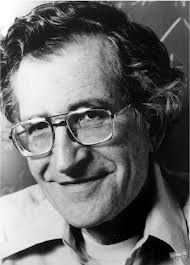
\includegraphics[width=1.0 in]{../images/Chomsky} \begin{minipage}[b]{8in} Noam Chomsky: 
  By the no free lunch theorem {\bf natural language grammar is unlearnable without an innate linguistic capacity}. In any domain a strong prior (a learning bias)
  is required. \end{minipage}

\vfill
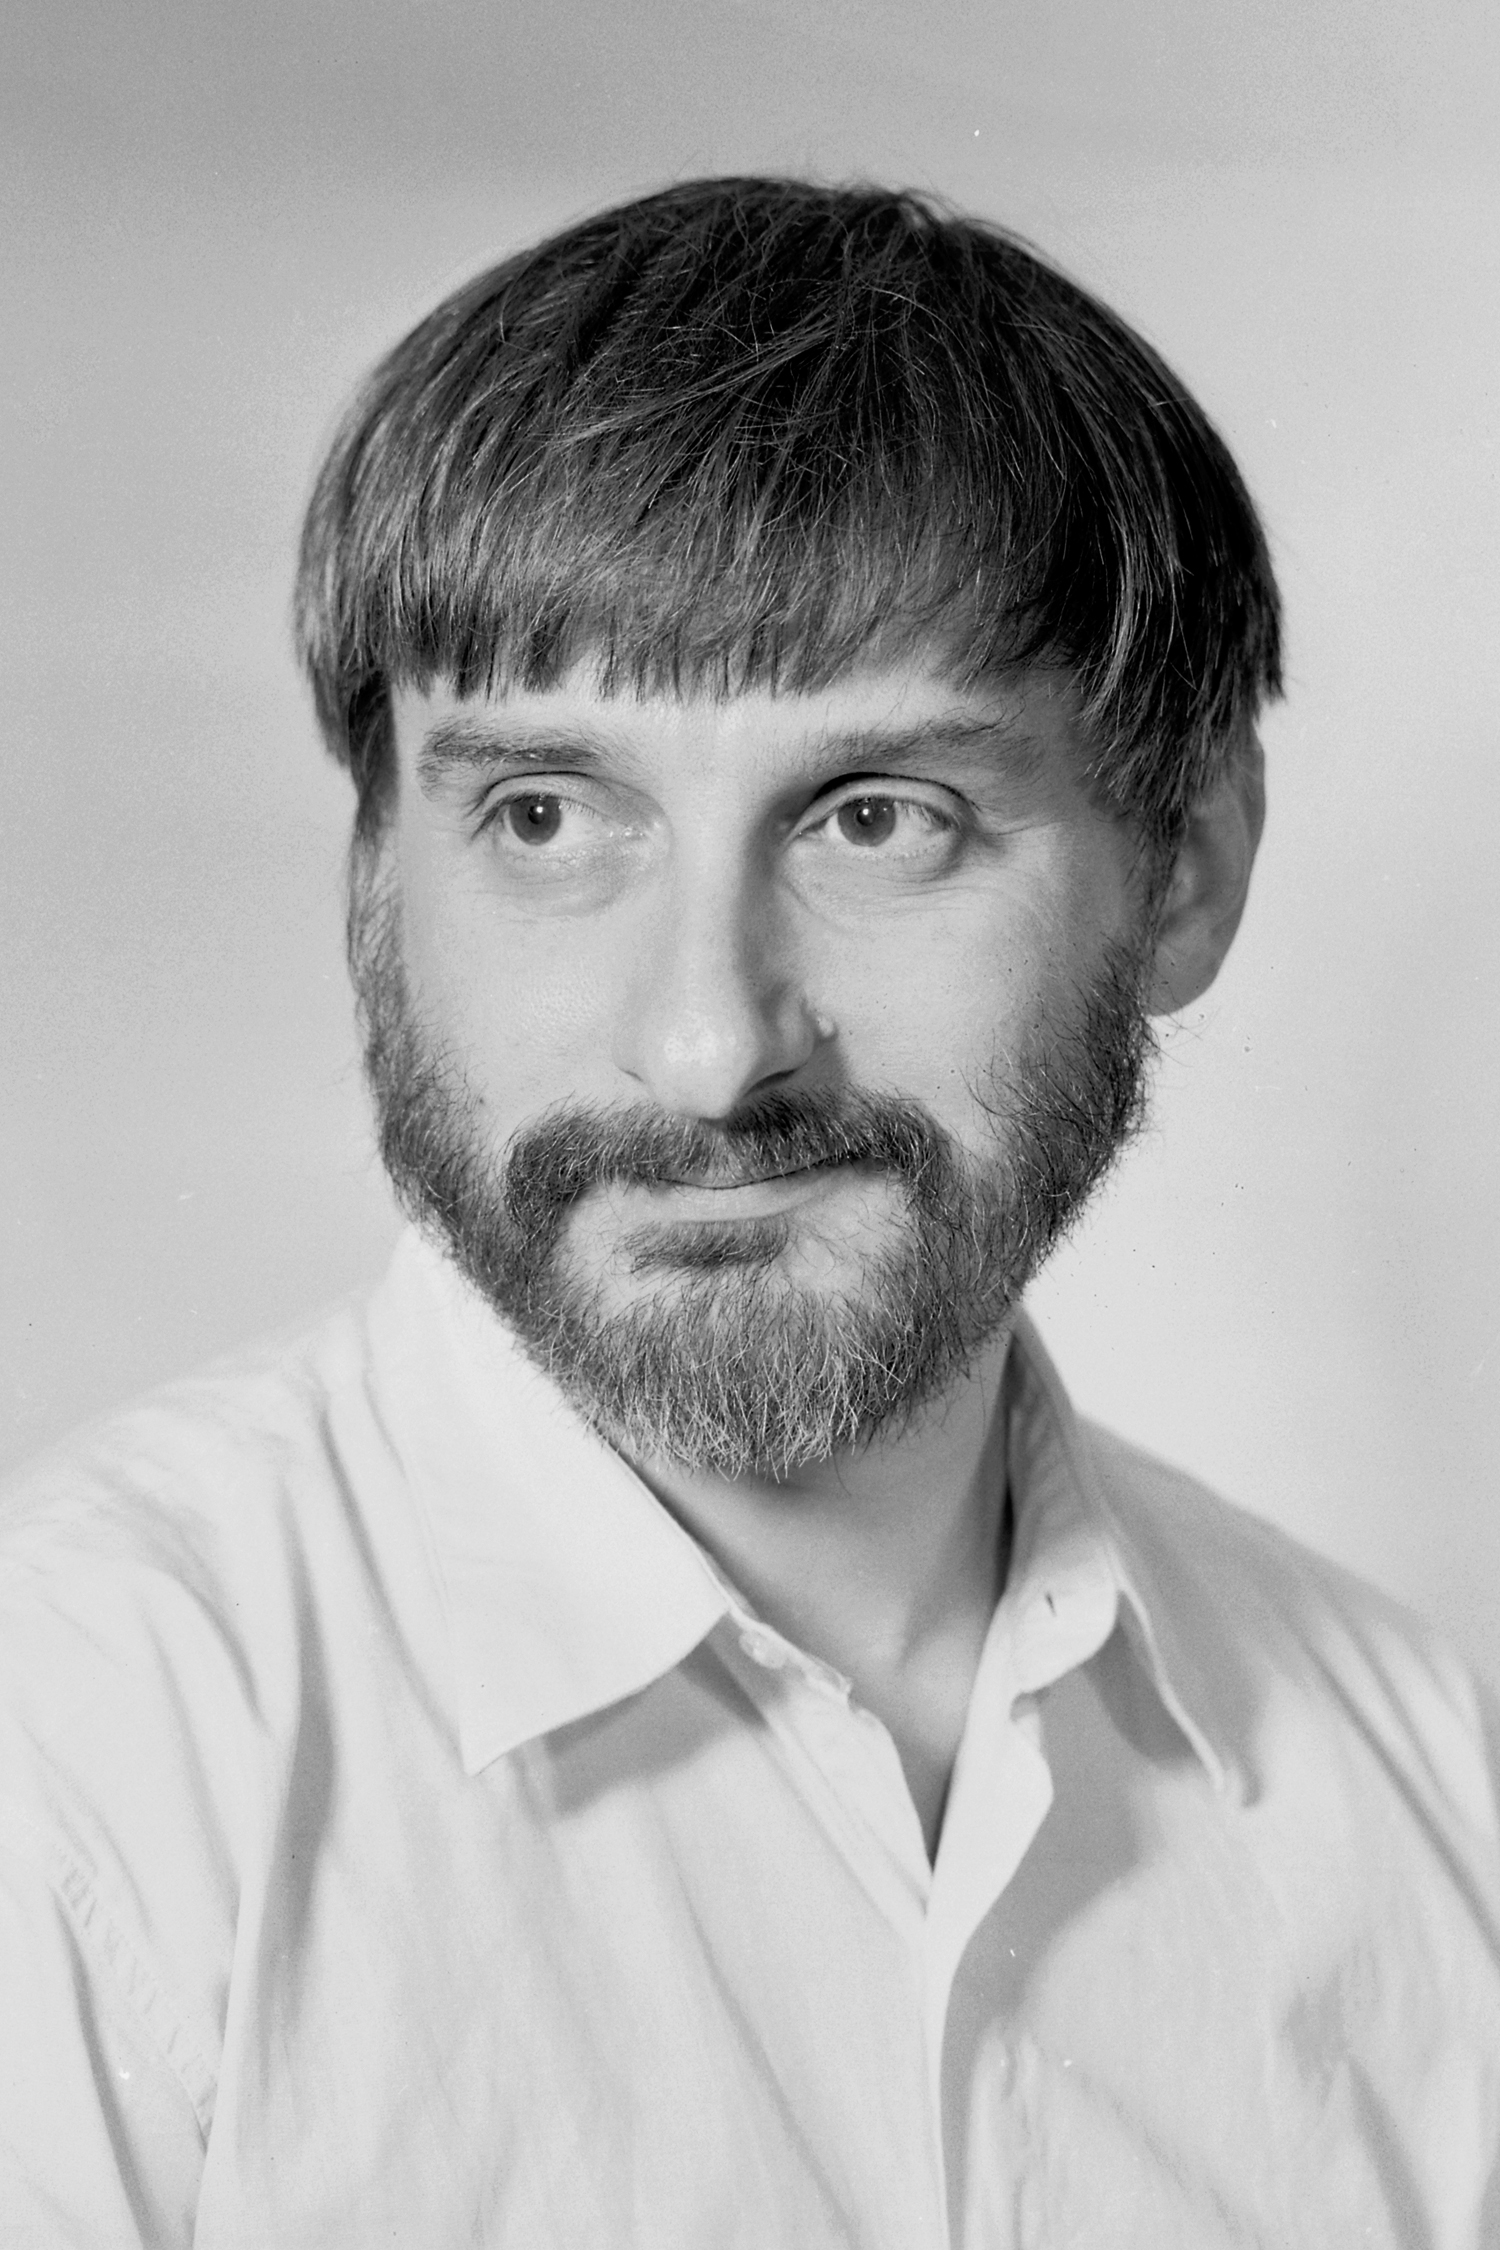
\includegraphics[height=1.0 in]{../images/Levin}
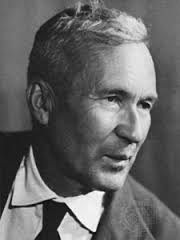
\includegraphics[height=1.0 in]{../images/Kolmogorov}
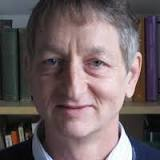
\includegraphics[height=1.0 in]{../images/Hinton}
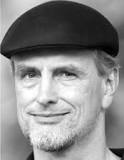
\includegraphics[height=1.0 in]{../images/Schmidhuber}

\begin{minipage}[b]{7in}
  Leonid Levin, Andrey Kolmogorov, Geoff Hinton and J\"{u}rgen Schmidhuber: {\bf Universal learning algorithms exist.
  No domain-specific innate knowledge is required.}
\end{minipage}


\slide{Is Domain-Specific Insight Valuable?}

\vfill
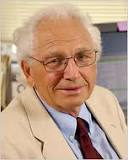
\includegraphics[width=1.0 in]{../images/Jelinek} \begin{minipage}[b]{8in}
Fred Jelinek: Every time I fire a linguist our recognition rate improves.
\end{minipage}
\vfill
\vfill

\slide{C++ as a Universal Architecture}

Let $h$ be any C++ procedure that can be run on a problem instance to get a loss where the loss is scaled to be in $[0,1]$.

\vfill
Let $|h|$ be the number of bits in the Zip compression of $h$.

\vfill
{\bf Free Lunch Theorem:} With probability at least $1-\delta$ over the draw of the sample the following holds {\em simultaneously} for all C++ programs $h$
and all $\lambda > 1/2$.
$$\ell(h) \leq \frac{1}{1-\frac{1}{2\lambda}}\parens{\widehat{\ell}(h) + \frac{\lambda}{N}\parens{(\ln 2)|h| + \ln\frac{1}{\delta}}}$$


\slide{The Turing Tarpit}

The choice of programming language does not matter.

\vfill
For any two Turing universal languages $L_1$ and $L_2$ there exists a compiler $C: L_1 \rightarrow L_2$ such that

$$|C(h)| \leq |h| + |C|$$

\slide{(Differentiable) Universal  Computation}

The Circuit Model

\vfill
The Von Neumann Architecture (``Neural Turing Machines'')

\vfill
Functional Programming

\vfill
Logic Programming

\slide{Universal Knowledge Representation}

Knowledge Graphs (Freebase, Wikidata)

\vfill
Natural Language as Knowledge Representation

\vfill
The Foundations of Mathematics

\vfill
The Concept of Truth.

\slide{Universal Function Representation Theorems}

Consider continuous functions $f: [0,1]^N \rightarrow \reals$

\vfill
\vfill
\centerline{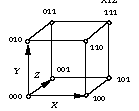
\includegraphics[width = 2in]{../images/n-cube} 
\begin{minipage}[b]{2.0in}
  $\stackrel{f}{\rightarrow} \;\;\;\reals$ \newline
  \vspace{2ex}
\end{minipage}}

\vfill
Given the corner values, the interior can be filled.

$$f(x_1,\ldots,x_N) = \prod_{y_1,\ldots,y_n,\;y_i \in \{0,1\}} f(y_1,\ldots,y_n) \prod_{i=1}^N (x_iy_i + (1-x_i)(1-y_i))$$

\vfill
Hence each of the $2^N$ corners has an independent value.

\slide{The Kolmogorov-Arnold representation theorem (1956)}

For continuous $f: [0,1]^N \rightarrow \reals$ there exists continuous
$g_i,h_{i,j} : \reals \rightarrow \reals$ such that


\vfill
$$f(x_1,\;\ldots,\;x_N)=\sum _{{i=1}}^{{2N+1}} g_i \left(\sum_{j=1}^N\;h_{i,j}(x_j)\right)$$

\vfill
$$f(x_1,x_2) = \left\{\begin{array}{ll}& g_1(h_{1,1}(x_1) + h_{1,2}(x_2)) \\ + & g_2(h_{2,1}(x_1) + h_{2,2}(x_2)) \\ \vdots \\ + & g_5(h_{5,1}(x_1) + h_{5,2}(x_2))\end{array}\right.$$


\slide{A Simpler, Similar Theorem}

For (possibly discontinuous) $f: [0,1]^N \rightarrow \reals$ there exists (possibly discontinuous)
$g, h_i: \reals \rightarrow \reals$.

\vfill
$$f(x_1,\;\ldots,\;x_N) = g\left(\sum_i h_i(x_i)\right)$$

\vfill
Proof: Select $h_i$ to spread out the digits of its argument so that $\sum_i h_i(x_i)$ contains all the digits of all the $x_i$.

\slide{Cybenko's Universal Approximation Theorem (1989)}

For continuous $f: [0,1]^N \rightarrow \reals$ and $\varepsilon >0$ there exists

\vfill
\begin{eqnarray*}
  F(x) &= & \alpha^\top \sigma(Wx + \beta) \\
  \\
  & = & \sum_i \alpha_i \sigma\left(\sum_j W_{i,j} \;x_j + \beta_i\right)
\end{eqnarray*}


\vfill
such that for all $x$ in $[0,1]^N$ we have $| F( x ) - f ( x ) | < \varepsilon$.

\slide{How Many Hidden Units?}

Consider Boolean functions $f:\;\{0,1\}^N \rightarrow \{0,1\}$.

\vfill
For Boolean functions we can simply list the inputs $x^0,\;\ldots,\;x^k$ where the function is true.

\begin{eqnarray*}
  f(x) & = & \sum_k \mathbbm{1}[x=x^k] \\
  \\
  \mathbbm{1}[x = x^k] & \approx & \sigma\left(\sum_i W_{k,i} x_i + b_k\right)
\end{eqnarray*}

\vfill
A simpler statement is that any Boolean function can be put in disjunctive normal form.

\slide{Circuit Complexity theory}

Building on work of Ajtai, Sipser and others, Hastad proved (1987) that any bounded-depth Boolean circuit computing the parity function must have exponential size. 

\vfill
Matus Telgarsky recently gave some formal conditions under which shallow networks provably require exponentially more parameters than deeper networks (COLT 2016).

\slide{Neural Turing Machines (NTM)}

Neural Turing Machines
Alex Graves, Greg Wayne, Ivo Danihelka, 2014

\vfill
(Actually a differentiable Von Neumann architecture)

\vfill
\centerline{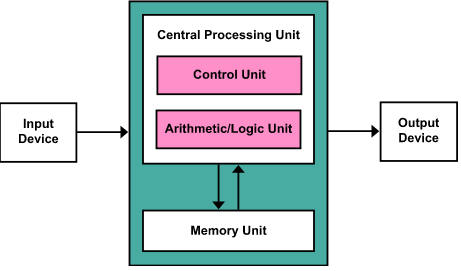
\includegraphics[width = 6in]{../images/VNA}}

\slideplain{CPU Registers of the NTM}

The CPU has a system of registers each of which stores a vector rather than a bit string.

\vfill
All computation is differentiable.

\vfill
Address registers (heads) hold an attention vector over all memory cells.

\vfill
Read address registers are separate from write address registers.

\slide{An Execution Cycle}

\vfill
The CPU receives an external input.

\vfill
The first step is to recompute the attention vectors in the read address registers.

\vfill
The CPU computes a ``key'' $k^h$ for each head $h$ and an attention $\alpha_j^h$

\begin{eqnarray*}
  \alpha^h_j & = & \softmax_j\;k^h \cdot M[j] \\
  \\
  r^h & = & \sum_j \alpha_j^h M[j]
\end{eqnarray*}

\slide{Reading from Memory}

Once the read address vectors (attentions) have been computed we read a value for each read head.

\vfill
$$v^h = \sum_j \;\alpha^h_j M[j]$$

After reading from memory the machine computes a key and attention for each write head.

\vfill
Each write operation involves ``forget'' and ``input'' operation analogous to an LSTM.

\vfill
Finally the controller emits an external output vector.

\slide{Neural Programmer Interpreter}

Neural Programmers-Interpreter, Scott Reed and Nando de Freitas, ICLR, 2016

\slide{Neural Programmer Interpreter}

We will use
\begin{eqnarray*}
i &\sim & \mbox{procedure pointer (integer)} \\
p &\sim & \mbox{procedure instruction (vector)} \\
a &\sim & \mbox{arguments (sequence of integers)} \\
e &\sim& \mbox{memory (array of vectors)} \\
h & \sim& \mbox{CPU state vector}
\end{eqnarray*}

To execute a procedure call $\mathrm{RUN}(i,a,e)$

\vfill
\begin{quotation}
$h \leftarrow 0$

$p \leftarrow  M^{\mathrm{Prog}}[i]$

\vfill
Until $f_{\mathrm{end}}(h): \;\;\;e,h \leftarrow \mathrm{DoStep}(p,a,e,h)$

\vfill
$\mathrm{return}(e)$
\end{quotation}

\slide{DoStep}

To compute $\mathrm{DoStep}(p,a,e,h)$

\vfill
\begin{quotation}
$h \leftarrow f_{\mathrm{LSTM}}(p,a,e,h)$

\vfill
$k \leftarrow f_{\mathrm{prog}}(h)$

\vfill
$i \leftarrow \argmax_i\; k^\top M^{\mathrm{Key}}[i]$

\vfill
If $i = 0:\;\;e \leftarrow f_{\mathrm{Env}}(p,f_{\mathrm{Arg}}(h),e)$

\vfill
else: $e \leftarrow \mathrm{RUN}(i,f_\mathrm{Arg}(h),e)$

\vfill
$\mathrm{return}(e,h)$
\end{quotation}


\slide{Non-Differentiable Steps}

To execute a procedure call $\mathrm{RUN}(i,a,e)$

\vfill
\begin{quotation}
$h \leftarrow 0$

$p \leftarrow  M^{\mathrm{Prog}}[i]$

\vfill
Until ${\color{red} f_{\mathrm{end}}(h)}: \;\;\;e,h \leftarrow \mathrm{DoStep}(p,a,e,h)$

\vfill
$\mathrm{return}(e)$
\end{quotation}

\slide{Non-Differentiable Steps}

To compute $\mathrm{DoStep}(p,a,e,h)$

\vfill
\begin{quotation}
$h \leftarrow f_{\mathrm{LSTM}}(p,a,e,h)$

\vfill
$k \leftarrow f_{\mathrm{prog}}(h)$

\vfill
$i \leftarrow {\color{red} \argmax_i}\; k^\top M^{\mathrm{Key}}[i]$

\vfill
If $i = 0:\;\;e \leftarrow f_{\mathrm{Env}}(p,{\color{red} f_\mathrm{Arg}(h)},e)$

\vfill
else: $e \leftarrow \mathrm{RUN}(i,{\color{red} f_\mathrm{Arg}(h)},e)$

\vfill
$\mathrm{return}(e,h)$
\end{quotation}

\slide{Training on Execution Traces}

To train they use execution traces

\vfill
$$e_t, i_t, a_t \Rightarrow  i_{t+1},a_{t+1},f_{\mathrm{end}}$$

\slide{Tail Recursion}

\vfill
Making Neural Programming Architectures
Generalize Via Recursion, Jonathon Cai, Richard Shin, Dawn Song, ICLR, 2017

\vfill
Allowing tail recursion, and explicitly labeling tail recursions in traces, significantly improves learning.

\slide{Bottom-up Logic Programming}

Bottom-up logic programming is distinguished by its relationship to dynamic programming algorithms.

\vfill
$$\mathrm{At}(x) \Rightarrow \mathrm{Reachable}(x)$$

\vfill
$$\mathrm{Reachable}(x) \wedge \mathrm{Edge}(x,y) \Rightarrow \mathrm{Reachable}(y)$$

\vfill
This defines a linear time algorithm for reachability.

\slide{The CKY algorithm for context-free parsing}

Consider a grammar defined by productions of the form $S \rightarrow \mathrm{NP}\;\mathrm{VP}$ and $N \rightarrow \mathrm{Kelly}$.

\vfill
The $O(n^3)$ CKY parsing algorithm is defined by the following two rules.

$$X \rightarrow a \;\;\wedge \;\; S[i] = a \;\; \Rightarrow X[i,i+1]$$

\vfill
$$X \rightarrow YZ \;\;\wedge \;\; Y[i,j]\;\; \wedge \;\; Z[j,k] \;\;\Rightarrow X[i,k]$$

\slide{Datalog}

A set of inference rules each of which has antecedents and conclusions that are just predicates applied to variables is called a {\bf datalog} program.

\vfill
It can be shown that datalog ``captures the complexity class $P$'' --- they can express {\bf all and only} polynomial time decidable relations
(provided the entities are assigned a total order).

\vfill
General bottom-up logic programs, including expressions (terms), are Turing complete.

$$N(x) \Rightarrow N(s(x))$$

\slide{Universal Knowledge Representation}

Knowledge Graphs (Freebase, Wikidata)

\vfill
Natural Language as Knowledge Representation

\vfill
The Foundations of Mathematics

\vfill
The Concept of Truth.

\slide{Natural Language Semantics}

Thousands of civilians have fled advances by Syrian government forces in eastern Ghouta as ...

\slide{Stanford Parse Tree}
\begin{verbatim}
(NP (NP (NNS Thousands))
    (PP (IN of) (NP (NNS civilians))))
(VP (VBP have)
    (VP (VBN fled)
        (NP (NNS advances))
        (PP (IN by) (NP (NP (JJ Syrian)
                            (NN government)
                            (NNS forces))
                        (PP (IN in) (NP (JJ eastern)
                                        (NNP Ghouta))))))))
\end{verbatim}

\slideplain{Stanford Dependencies}

\begin{verbatim}
root(ROOT-0, fled-5)
  aux(fled-5, have-4)
  nsubj(fled-5, Thousands-1)
    nmod(Thousands-1, civilians-3)
      case(civilians-3, of-2)
  dobj(fled-5, advances-6)
  nmod(fled-5, forces-10)
    case(forces-10, by-7)
    amod(forces-10, Syrian-8)
    compound(forces-10, government-9)
    nmod(forces-10, Ghouta-13)
      case(Ghouta-13, in-11)
      amod(Ghouta-13, eastern-12)
\end{verbatim}

\slideplain{Just Parantheses}

\begin{verbatim}
(Thousands of civilians)
(have fled)
(advances (by (Syrian government forces))
          (in eastern Ghouta))
\end{verbatim}

\slideplain{Reference}

{\color{blue} Thousands of civilians have fled advances by Syrian government forces in eastern Ghouta as}
Damascus makes rapid gains against the last major rebel enclave near the capital.

\vfill
Damascus $\Rightarrow$ Assad

\vfill
Rapid Gains $\Rightarrow$ advances-6

\vfill
the last major rebel enclave ... $\Rightarrow$ Ghouta

\vfill
the capital $\Rightarrow$ Damascus

\slide{Reference vs. Composition}

Functional Programming is compositional

\vfill
$$x = f(y,z)$$

\vfill
The meaning of $x$ is computed by $f$ from the meaning of $y$ and $z$.

\vfill
But in language we typically have that $f(y,z)$ is a mention and $x$ is its referent.

\vfill
(the last (major rebel enclave) (near (the capital)))

\vfill
$$x = (\mbox{the last $Q$ $P$})$$

\slide{Natural Language: Parsing}

A Fast and Accurate Dependency Parser using Neural Networks,
Danqi Chen and Christopher Manning, 2014.

\vfill
$$\begin{array}{lllll}
  \vdots \\
  s_3 \\
    s_2 \\
    s_1 \\
    * & b_1 & b_2 & b_3 & \ldots
  \end{array}
  \;\;\;\;
  \stackrel{\mbox{push}}{\Rightarrow}
  \;\;\;
  \begin{array}{lllll}
    \vdots \\
    s_2 \\
    s_1 \\
    b_1 \\
    * & b_2 & b_3 & b_4 & \ldots
  \end{array}$$

\slide{Arc Transitions}

$$\begin{array}{llll}
    \begin{array}{lllll}
      \vdots \\
      s_3 \\
    s_2 \\
    s_1 \\
    * & b_1 & b_2 & b_3 & \ldots
  \end{array}
  &
  \stackrel{\mbox{LeftArc}}{\Rightarrow}
  &
  \begin{array}{lllll}
    \vdots \\
    s_4 \\
    s_3 \\
    s_1 \\
    * & b_1 & b_2 & b_3 & \ldots
  \end{array}
  &
  \mbox{Emits} \;s_1 \stackrel{\ell}{\rightarrow} s_2 \\
  \\
  \\
    \begin{array}{lllll}
      \vdots \\
      s_3 \\
    s_2 \\
    s_1 \\
    * & b_1 & b_2 & b_3 & \ldots
  \end{array}
  &
  \stackrel{\mbox{LeftArc}}{\Rightarrow}
  &
  \begin{array}{lllll}
    \vdots \\
    s_4 \\
    s_3 \\
    s_2 \\
    * & b_1 & b_2 & b_3 & \ldots
  \end{array}
  &
  \mbox{Emits} \;s_2 \stackrel{\ell}{\rightarrow} s_1 \\
\end{array}
$$

\slide{Dependency Parsing Machine Configurations}

A machine configuration

$$c = (s,b,A)$$

\begin{eqnarray*}
  s & \sim & \mbox{stack} \\
  \\
  b & \sim & \mbox{buffer} \\
  \\
  A & \sim & \mbox{Dependency Arcs}
\end{eqnarray*}

\slide{Training}

Construct a database of machine configurations labeled with actions.

\vfill
Train an MLP with one hidden layer to a softmax over actions and train on cross entropy.

\vfill
The input to the MLP is a concatenation of 18 word vectors defined in terms of the configuration

\vfill
plus 18 corresponding part of speech vectors

\vfill
and 12 parent edge label vectors.


\slide{The Foundations of Mathematics}

  $$
  \begin{array}{lccccccc}
    \mbox{variables, pairs} & x & (e_1,e_2) & \pi_i(e) \\ \\
    \mbox{functions} & \lambda \intype{x}{\sigma}\;e[x] & f(e) \\ \\
    \mbox{Booleans} & ~~~~~~~P(e)~~~~~~~ & ~~~~~~~~ e_1 \doteq e_2 ~~~~~~~~ & ~~~~~~~~e_1 =_\sigma e_2 ~~~~~~~~ \\ \\
    & \neg \Phi &  \Phi_1 \vee \Phi_2 & \forall \intype{x}{\sigma}\; \Phi[x] \\ \\
    \mbox{types}   & \Sigma_{\intype{x\;}{\;\sigma}}\;\tau[x] & \Pi_{\intype{x\;}{\;\sigma}}\;\tau[x] & S_{\intype{x\;}{\;\sigma}}\;\Phi[x]
  \end{array}
  $$

\slide{The Base Case}

The base case is given by $\bool$, $\mathbf{Set}$ and $\mathbf{Type}$ with $\intype{\bool}{\mathbf{Type}}$ and $\intype{\mathbf{Set}}{\mathbf{Type}}$.


\begin{eqnarray*}
\sigma \times \tau & \doteq & \Sigma_{\intype{\alpha\;}{\;\sigma}}\;\tau \;\;\;\alpha\;\mbox{not in}\;\tau\\
\\
\\
\mathbf{Graph} & \doteq & \Sigma_{\intype{\alpha\;}{\;\mathbf{Set}}}\;(\alpha \times \alpha) \rightarrow \bool
\end{eqnarray*}

\slide{Learning Guiding Evolution}

\includegraphics[width = 1.2in]{../images/hinton}

In a 1987 paper entitled ``How Learning Can Guide Evolution'', Goeffrey Hinton and Steve Nowlan brought attention to a paper by Baldwin (1896).

\vfill
The basic idea is that learning facilitates modularity.

\vfill
For example, longer arms are easier to evolve if arm control is learned --- arm control is then independent of arm length.  Arm control and arm structure become more modular.

\slide{Learning Guiding Learning}

\vfill
If each ``module'' is learning to participate in the ``society of mind'' then each model can more easily accommodate (exploit) changes (improvements) in other modules.

\vfill
Modularity (and abstraction) are fundamental principle of software design.

\slide{Levin's Universal Problem Solver (Levin Search)}

Leonid Levin observed that one can construct a universal solver that takes as input an oracle for testing proposed solutions
and, if a solution exists, returns it.

\vfill
One can of course enumerate all candidate solutions.

  \vfill
However, Levin's solver is universal in the sense that it is not more than a constant factor slower than any other solver.


\slide{Levin's Universal Solver}
  
\vfill
We time share all programs giving time slice $2^{-|h|}$ to program $h$ where $|h|$
is the length in bits of $h$.

\vfill
The run time of the universal solver is at most
$$O(2^{-|h|}(h(n) + T(n)))$$
where $h(n)$ is the time required to run program $h$ on a problem of size $n$ and $T(n)$ is the time required to check the solution.

\vfill
Here $2^{-|h|}$ is independent of $n$ and is technically a constant.

\slide{Bootstrapping Levin Search}

\includegraphics[width= 1in]{../images/schmidhuber}

While Levin search sounds like a joke, Schmidhuber takes it seriously.

\vfill
He has proposed ways of accelerating a search over all programs and has something called the Optimal Ordered Problem Solver (OOPS).

\vfill
The basic idea is bootstrapping --- we automate a search for methods of efficient search.

\slide{END}

}
\end{document}
